% !Mode:: "Tex:UTF-8"


Ahora que ya sabemos resumir la información de los datos en tablas y
presentarlos gráficamente, vamos a dar un paso más. Vamos a sintetizar esa
información en un número, que llamaremos ``valor central''. Una de las ideas centrales de este capítulo es que ese valor central tiene que ser un buen representante del conjunto de datos que estamos usando. También veremos que, como no podía ser de otra manera, la elección del representante adecuado depende de la tarea para la que lo vayamos a utilizar. \\
Pero además, una vez elegido un representante de un conjunto de datos,
querremos saber cómo de representativo es ese valor central, respecto del
conjunto de datos que describe. Eso nos llevará a hablar de la idea de
dispersión. La dispersión es, precisamente, una medida de la calidad del valor
central, como representante de un conjunto de datos. Es una noción directamente
emparentada con la idea de precisión, de la que hablamos en el capítulo
anterior (ver Figura \ref{cap01:fig:PrecisionExactitud} en la pág.
\pageref{cap01:fig:PrecisionExactitud}).

\section{La media aritmética.}
\label{cap02:sec:MediaAritmetica}

Vamos a aprovechar este concepto, que suponemos ya conocido del lector, para
introducir parte de la notación abstracta, típica de las Matemáticas, que
utilizaremos a lo largo del curso. Esta sección puede servir de ``chequeo
preliminar'' para el lector. Si tienes muchas dificultades con la notación en
este punto inicial del curso, es probable que necesites reforzar tus
habilidades matemáticas para poder seguir adelante. En los tutoriales 1 y 2 aprenderemos, entre otras cosas, a realizar estos cálculos en el ordenador.

\subsection{Definición de la media aritmética.}
\label{cap02:subsec:DefincionMediaAritmetica}

La idea de media aritmética apenas necesita presentación. Dados $n$ valores de una {\sf variable
cuantitativa}, sean $x_1,x_2,\ldots,x_n$, su {\sf media aritmética} \index{media aritmética} (en
inglés, {\em arithmetic mean} o {\em average}) \index{mean}\index{arithmetic mean}\index{average}
es:
    \begin{center}
        \fcolorbox{black}{Gris025}{\begin{minipage}{8cm}
        %\centering{\bf Media aritmética: }
            \begin{equation}
            \label{cap02:ecu:MediaAritmetica}
            \bar x=\dfrac{x_1+\cdots+x_n}{n}=\dfrac{\displaystyle\sum_{i=1}^nx_i}{n}.
            \end{equation}
    \end{minipage}}
    \end{center}
Algunos comentarios sobre la notación. El símbolo $\bar x$ refleja la notación establecida en Estadística: la media de un vector de datos se representa con una barra sobre el nombre de ese vector. Y el símbolo $\displaystyle\sum_{i=1}^n x_i$, que suponemos que el lector ya conoce, es un {\sf sumatorio}, \index{sumatorio} y representa en forma abreviada, la frase ``suma todos estos valores $x_i$ donde $i$ es un número que va desde 1 hasta $n$''.

Insistimos en esto: la {\bf media aritmética sólo tiene sentido para variables
cuantitativas} (discretas o continuas). Aunque una variable cualitativa se
represente numéricamente, la media aritmética de esos números seguramente sea
una cantidad sin ningún significado estadístico.

La media aritmética es ``la media'' por excelencia. Pero hay otros conceptos de
media que juegan un papel importante en algunos temas: la media geométrica, la
media armónica, etc. Pero no las vamos a necesitar en este curso, así que no
entraremos en más detalles.

\begin{ejemplo}
\label{cap02:ejem:MediaAritmetica}
Dado el conjunto de valores (son $n=12$ valores)
\[9,\, 6,\, 19,\, 10,\, 17,\, 3,\, 28,\, 19,\, 3,\, 5,\, 19,\, 2,\]
su media aritmética es:
{\scriptsize
\[\bar x=\dfrac{9 + 6 + 19 + 10 + 17 + 3 + 28 + 19 + 3 + 5 + 19 + 2}{12}=\]
}
\[=\dfrac{140}{12}\approx 11.67,\]
(cuatro cifras significativas). Proponemos al lector como ejercicio que piense si el número $\bar x=11.67$ se puede considerar, en este caso, un buen representante de este conjunto de datos.
\qed
\end{ejemplo}

El siguiente ejemplo sirve para presentar una característica de la media aritmética que debemos tener siempre presente:
\begin{ejemplo}
\label{cap02:ejem:MediaAritmetica02}
Ahora consideramos el mismo conjunto de valores, al que añadimos el número $150$ (en la última posición, aunque su posición es irrelevante para lo que sigue):
\[9,\, 6,\, 19,\, 10,\, 17,\, 3,\, 28,\, 19,\, 3,\, 5,\, 19,\, 2,\, 150\]
La media aritmética ahora es:
{\scriptsize
\[\bar x=\dfrac{9 + 6 + 19 + 10 + 17 + 3 + 28 + 19 + 3 + 5 + 19 + 2 + 150}{13}=\]
}
\[=\dfrac{290}{13}\approx 22.31,\]
(con cuatro cifras significativas). ¿Sigue siendo posible, en este caso, considerar a la media aritmética $\bar x=22.31$ como un buen representante de los datos? Por ejemplo, si elegimos al azar uno cualquiera de esos números, ¿es de esperar que se parezca a la media?
\qed
\end{ejemplo}
Volveremos sobre la pregunta que plantean estos ejemplos en la Sección \ref{cap02:sec:MedianaCuartilesPercentilesModa} (pág. \pageref{cap02:sec:MedianaCuartilesPercentilesModa}). Pero antes vamos a pensar un poco más sobre la forma de calcular la media aritmética, si los datos vienen descritos mediante una tabla de frecuencias.


\subsection{La media aritmética a partir de una tabla de frecuencias.}
\label{cap02:subsec:MediaAritmeticaAPartirTablaFrecuencias}


    Supongamos que tenemos una tabla de frecuencias de unos valores, correspondientes a una variable cuantitativa. Es decir, una tabla como esta :
   \begin{center}
        \begin{tabular}{|c|c|}
        \hline
        \rule{0cm}{4mm}{\bf Valor}&{\bf Frecuencia}\\ \hline
        \rule{0cm}{4mm}$x_1$&$f_1$\\[2mm] \hline
        \rule{0cm}{4mm}$x_2$&$f_2$\\[2mm] \hline
        $\vdots$&$\vdots$\\[2mm] \hline
        \rule{0cm}{4mm}$x_k$&$f_k$\\[2mm] \hline
        \end{tabular}
        \end{center}
   y  queremos calcular la media aritmética a partir de esta tabla.

   Aquí los valores {\em distintos} de la variable\footnote{Acuérdate de que tenemos $n$ observaciones de la variable, pero puede haber valores repetidos. Aquí estamos usando el número de valores distintos, sin repeticiones, y ese número es $k$.} son $x_1,\ldots,x_k$ y sus frecuencias absolutas respectivas son $f_1,f_2,\ldots,f_k$. Está claro entonces que:
        \[f_1+f_2+\cdots+f_k=(\mbox{núm. de observ. de }x_1)+\cdots+(\mbox{núm. de observ. del valor }x_k)= \]
        \[=(\mbox{suma del número de observaciones de todos los valores distintos})=n\]
        Recordemos que para calcular la media tenemos que sumar el valor de todas (las $n$ observaciones). Y como el valor $x_i$ se ha observado $f_i$ veces, su contribución a la suma es
        \[x_i\cdot f_i=x_i+x_i+\cdots+x_i\quad (\mbox{sumamos $f_i$ veces})\]
        Teniendo en cuenta la contribución de cada uno de los $k$ valores distintos, vemos que
        para calcular la media debemos hacer:
%       \begin{center}
%        \fbox{\colorbox{Gris025}{
%            \begin{minipage}{8cm}
%            {\[
%        \bar x=\dfrac{x_1\cdot f_1+x_2\cdot f_2+\cdots+x_k\cdot f_k}{f_1+f_2+\cdots+f_k}=
%        \dfrac{\displaystyle\sum_{i=1}^k x_i\cdot f_i}{\displaystyle\sum_{i=1}^k f_i}\]}
%           \end{minipage}}
%        }
%        \end{center}
        \begin{center}
                \fcolorbox{black}{Gris025}{\begin{minipage}{8cm}
                	    \[\bar x=\dfrac{x_1\cdot f_1+x_2\cdot f_2+\cdots+x_k\cdot f_k}{f_1+f_2+\cdots+f_k}=
                        \dfrac{\displaystyle\sum_{i=1}^k x_i\cdot f_i}{\displaystyle\sum_{i=1}^k f_i}.\]
        \end{minipage}}
        \end{center}


        \begin{Ejemplo}
        En una instalación deportiva el precio de la entrada para adultos es de \EUR{10} y de \EUR{4} para menores. Hoy han visitado esa instalación $230$ adultos y $45$ menores. ¿Cuál es el ingreso medio por visitante que recibe esa instalación?\\
        Tenemos dos posibles valores de la variable $x=${\em ``precio de la entrada''}, que son $x_1=10$ y $x_2=4$. Además sabemos las frecuencias correspondientes: $f_1=230$ y $f_2=45$. Por lo tanto:
        \[\bar x=\dfrac{x_1\cdot f_1+x_2\cdot f_2}{f_1+f_2}=\dfrac{10\cdot 230+4\cdot 45}{230+45}=9.02\]
        El ingreso medio es de \EUR{9.02} por visitante.\qed
        \end{Ejemplo}

    \subsection{Media aritmética con datos agrupados.}
    \label{cap02:subsec:MediaAritmeticaConDatosAgrupados}

    Si lo que queremos es calcular la media aritmética a partir de la tabla de frecuencias agrupadas por intervalos de una variable cuantitativa (ver el final de la Sección \ref{cap01:subsec:NotacionVariablesTablasFrecuenciaDatosAgrupados}), las cosas son (sólo un poco)  más complicadas. En este caso vamos a tener una tabla de frecuencias por intervalos (recuerda que los intervalos a veces se llaman también {\sf clases}) como esta:
        \begin{center}
        \begin{tabular}{|c|c|}
        \hline
        \rule{0cm}{4mm}{\bf Intervalo}&{\bf Frecuencia}\\ \hline
        \rule{0cm}{4mm}$[a_1,b_1)$&$f_1$\\[2mm] \hline
        \rule{0cm}{4mm}$[a_2,b_2)$&$f_2$\\[2mm] \hline
        $\vdots$&$\vdots$\\[2mm] \hline
        \rule{0cm}{4mm}$[a_k,b_k)$&$f_k$\\[2mm] \hline
        \end{tabular}
        \end{center}
        Comparando esta tabla con el caso anterior está claro que lo que nos falta son los valores $x_1,\ldots,x_k$ y, en su lugar, tenemos los intervalos $[a_1,b_1),\ldots,[a_k,b_k)$. Lo que hacemos en estos casos es {\em fabricar} unos valores $x_i$ a partir de los intervalos. Se toma como valor $x_i$ el punto medio del intervalo $[a_i,b_i)$; es decir:
%        \begin{center}
%        \fbox{\colorbox{Gris025}{
%            \begin{minipage}{6cm}
%            {
%        \[x_i=\dfrac{a_i+b_i}{2},\quad \text{ para } i=1,\ldots,n.\]}
%           \end{minipage}}
%        }
%        \end{center}
%%        \[\fbox{$x_i=\dfrac{a_i+b_i}{2}$,\quad para $i=1,\ldots,n.$}\]
        \begin{center}
                \fcolorbox{black}{Gris025}{\begin{minipage}{8cm}
                \begin{center}
                {\bf Marcas de clase.}
                \end{center}
                    \vspace{-3mm}
                    \begin{equation}
                    \label{cap02:ecu:MarcasDeClase}
                        x_i=\dfrac{a_i+b_i}{2},\quad \text{ para } i=1,\ldots,n.
                    \end{equation}
        \end{minipage}}
        \end{center}
        Estos valores $x_i$ se denominan {\sf marcas de clase} \index{marca de clase}
        \index{marca de intervalo} (o marcas de intervalo). Una vez calculadas las marcas de clase, podemos usar la misma fórmula que en el caso anterior.

\begin{ejemplo}
\label{cap02:ejem:MediaAritmeticaDesdeValoresAgrupadosClases}

La Tabla \ref{cap02:tabla:MediaAritmeticaValoresAgrupadosClases} muestra la tabla de frecuencias de un conjunto de $100$ datos agrupado por clases. En la última columna se muestran, además, las correspondientes marcas de clase.

\begin{table}[htp]
\begin{center}
\begin{tabular}{|l|c|c|}
  \hline
 Clase & Frecuencia & Marca de clase \\
  \hline
  [0,4) & 3 & 2 \\
  \hline
  [4,8) & 27 & 6 \\
  \hline
  [8,12) & 32 & 10 \\
  \hline
  [12,16) & 25 & 14 \\
  \hline
  [16,20) & 7 & 18 \\
  \hline
  [20,24) & 2 & 22 \\
  \hline
  [24,28] & 4 & 26 \\
  \hline
\end{tabular}
\label{cap02:tabla:MediaAritmeticaValoresAgrupadosClases}
\caption{Tabla de valores agrupados por clases del Ejemplo \ref{cap02:ejem:MediaAritmeticaDesdeValoresAgrupadosClases}}
\end{center}
\end{table}

\noindent A partir de la Tabla \ref{cap02:tabla:MediaAritmeticaValoresAgrupadosClases} es fácil calcular la media aritmética usando la Ecuación \ref{cap02:ecu:MarcasDeClase}:
\[
\bar x=\dfrac{3\cdot 2+27\cdot 6+32\cdot 10+25\cdot 14+7\cdot 18+2\cdot 22+4\cdot 26}{100}=
\dfrac{1112}{100}=11.12
\]
El fichero \fichero{../datos/Cap02-EjemploMediaAritmetica-ValoresAgrupadosClases.csv}{Cap02-EjemploMediaAritmetica-ValoresAgrupadosClases.csv} contiene los $100$ datos originales, sin agrupar por clases. Con los métodos que aprenderemos en los tutoriales es posible comprobar que la media aritmética de esos datos, calculada directamente, es, con seis cifras significativas, igual a $11.1158$. Así que, por un lado vemos que la media calculada a partir de los  datos agrupados no coincide con la media real. Pero, por otro lado, en ejemplos como este, el error que se comete al agrupar es relativamente pequeño.
\qed
\end{ejemplo}


\section{Mediana, cuartiles, percentiles y moda.}
\label{cap02:sec:MedianaCuartilesPercentilesModa}

Aunque la media aritmética es el valor central por excelencia, no siempre es la
que mejor refleja el conjunto de datos al que representa. La razón es, como hemos comprobado en el Ejemplo \ref{cap02:ejem:MediaAritmetica02} (pág. \pageref{cap02:ejem:MediaAritmetica02}), que la media es muy sensible a la presencia de valores mucho más grandes (o mucho más pequeños, tanto da) que la mayoría de los valores. Un nuevo ejemplo puede ayudar a reafirmar esta idea:
\begin{ejemplo}
\label{cap02:ejem:MediaConAtipicos}
Examinemos esta afirmación con un ejemplo muy sencillo. Los conjuntos de datos
	\[\left\{1,2,3,4,35\right\}\qquad \mbox{y} \qquad \left\{7,8,9,10,11\right\}\]
tienen la misma media, que vale $9$. Sin embargo, en el primer caso, el de la
izquierda, casi todos los valores son menores o iguales que $4$, y el hecho de
que aparezca un dato anormalmente alto, el $35$, aleja la media del grueso de
los datos. No ocurre así con la segunda serie de datos. Si jugamos con los
n\'umeros, pueden darse muchas situaciones diferentes.
\qed
\end{ejemplo}
Este ejemplo busca ponernos en guardia y motivar los conceptos que vamos a ver
continuación.


%\subsection*{Contenido:}
%\begin{itemize}
% \item Mediana.
% \item Moda
% %\item Opcional. Otras medias: media geométrica, armónica, etcétera.
%\end{itemize}


\subsection{Mediana.}
\label{cap02:subsec:Mediana}

Como en el caso de la media aritmética, vamos a suponer que tenemos $n$
observaciones de una variable cuantitativa
    \[x_1,x_2,\ldots,x_n.\]
y suponemos que los datos no están agrupados en una tabla de frecuencia. Más
abajo veremos el caso de datos agrupados.

Como los $x_i$ son números, vamos a suponer que los hemos ordenado de menor a
mayor:
    \[x_1\leq x_2\leq\cdots\leq x_{n-1}\leq x_n.\]
Entonces, la {\sf mediana}\index{mediana} (en inglés, {\em median})\index{median} de ese conjunto
de datos es el {\em valor central} de esa serie ordenada. Es decir:
    \begin{itemize}
        \item[]{\bf Caso impar:} si tenemos una cantidad impar de datos, sólo
            hay un valor central, y ese es la mediana. Por ejemplo, para
            siete datos:
                \[
                \begin{array}{rcl}
                \underbrace{x_1\leq x_2\leq x_3}_{\mbox{mitad izda.}}\leq &
                \hspace{-7mm}{\text{\Large{\bf x}}}_4 &\hspace{-7mm}\leq
                \underbrace{x_5\leq x_6\leq x_7}_{\mbox{mitad dcha.}}\\[-5mm]
                &\hspace{-7mm}\uparrow&\\
                &\hspace{-7mm}\colorbox{lightgrey}{\mbox{\small mediana}}&
                \end{array}
                \]

        \item[]{\bf Caso par:} por contra, si el número de datos es par,
            entonces tomamos el valor máximo de la mitad izquierda, y el
            valor mínimo de la mitad derecha y hacemos la media. Por ejemplo,
            para seis datos:
                \[
                \begin{array}{rcl}
                \underbrace{x_1\leq x_2\leq x_3}_{\mbox{mitad izda.}}\leq &\hspace{0mm}\colorbox{lightgrey}{$\dfrac{x_3+x_4}{2}$}&\hspace{0mm}\leq
                \underbrace{x_4\leq x_5\leq x_6}_{\mbox{mitad dcha.}}\\[-3mm]
                &\hspace{0mm}{\uparrow}&\\
                &\hspace{0mm}\colorbox{lightgrey}{\mbox{\small mediana}}&
                \end{array}
                \]

        \end{itemize}
En el caso de un número impar de datos la mediana siempre coincide con uno de
los datos originales. Pero en el caso de un número par de datos la mediana
pueden darse los dos casos.
\begin{ejemplo}
\label{cap02:ejem:CalculoMediana}
Por ejemplo, si tenemos estos seis datos ordenados:
        \[
        2\leq 5\leq 6\leq 7\leq 11\leq 15,
        \]
Entonces la mediana es $6.5$
        \[
        2\leq 5\leq 6\leq\colorbox{lightgrey}{\mbox{\Large\bf 6.5}}\leq 7\leq 11\leq 15,
        \]
que no aparecía en el conjunto original (fíjate en que, como pasaba con la
media aritmética, aunque todos los datos originales sean enteros, la mediana
puede no serlo). Mientras que si tenemos estos seis datos, con los dos datos
centrales iguales:
        \[
        2\leq 5\leq 6\leq 6\leq 11\leq 15,
        \]
Entonces la mediana es $6$,
        \[
        2\leq 5\leq 6\leq\colorbox{lightgrey}{\mbox{\Large\bf 6}}\leq 6\leq 11\leq 15,
        \]
que ya estaba (repetido) entre los datos originales.
\qed
\end{ejemplo}


¿Qué {\em ventajas} aporta la mediana frente a la media aritmética? Fundamentalmente, la mediana se
comporta mejor cuando el conjunto de datos contiene {\sf datos atípicos} \index{datos
atípicos}\index{atípico, dato} (en inglés, {\em outliers})\index{outliers}. Es decir, datos cuyo
valor se aleja {\em mucho} de la media. Todavía no podemos precisar esto porque para hacerlo
necesitamos un poco más de vocabulario que vamos a ver enseguida. Pero la idea intuitiva es que si
tenemos un conjunto de datos, e introducimos un dato adicional que se aleja mucho de la media
aritmética inicial, entonces en el nuevo conjunto de datos podemos tener una media aritmética
bastante distinta de la inicial. En cambio la mediana sufre modificaciones mucho menores frente a
esos datos atípicos. Podemos hacernos una primera impresión con un par de ejemplos, basados en
conjuntos de datos que ya hemos examinado antes.
\begin{ejemplo}
\label{cap02:ejem:MedianaVsMedia}
En el Ejemplo \ref{cap02:ejem:MediaAritmetica02} (pág. \pageref{cap02:ejem:MediaAritmetica02}) hemos visto que la media aritmética del conjunto de datos:
\[9,\, 6,\, 19,\, 10,\, 17,\, 3,\, 28,\, 19,\, 3,\, 5,\, 19,\, 2,\, 150\]
es
\[\bar x=\dfrac{290}{13}\approx 22.31.\]
Y, al comparar este resultado con el del Ejemplo \ref{cap02:ejem:MediaAritmetica}, hemos concluido que la presencia del valor $150$ (que es atípico, como veremos), tenía un efecto muy grande en la media aritmética, hasta el punto de hacerla poco útil como representante del conjunto de datos. Para calcular la mediana, empezamos por ordenar los datos de menor a mayor:
\[2,\, 3,\, 3,\, 5,\, 6,\, 9,\, 10,\, 17,\, 19,\, 19,\, 19,\, 28,\, 150.\]
Puesto que son $13$ números, la mediana es el valor que ocupa la séptima posición; es decir, la mediana vale $10$.  Y como se ve, es mucho más representativa de la mayoría de los números de este conjunto.

Además, veamos lo que sucede si eliminamos el valor $150$, para volver al conjunto de datos del Ejemplo \ref{cap02:ejem:MediaAritmetica} y, después de eliminarlo, volvemos  a calcular la mediana. Los datos restantes, ordenados, son estos $12$ números:
\[2,\, 3,\, 3,\, 5,\, 6,\, 9,\, 10,\, 17,\, 19,\, 19,\, 19,\, 28.\]
Y ahora la mediana será la media entre los números de la sexta y séptima posiciones. Por lo tanto la mediana es $9.5$. Como puede verse, el cambio en la mediana, debido a la presencia de $150$, es muy pequeño, comparado con el que sufre la media aritmética. Y, de hecho, si sustituimos $150$ por un valor aún más exagerado, como $2000$, veremos que la mediana cambia exactamente igual.
\end{ejemplo}
Como pone de manifiesto este ejemplo, {\em la mediana no atiende a tamaños, sino a posiciones}. Eso la hace muy adecuada para representar un conjunto de valores del que sospechamos que puede contener valores con tamaños muy alejados de los de la mayoría.
%Para observar otro ejemplo de este comportamiento se puede usar el fichero GeoGebra \fichero{../datos/Cap02-MediaMedianaAtipicos.ggb}{{Cap02-MediaMedianaAtipicos.ggb}}, y experimentar con él.

Y entonces, ¿por qué no se usa siempre la mediana en lugar de la media aritmética? La respuesta es que la Estadística basada en la mediana utiliza unas matemáticas bastante más complicadas que la que se basa en la media aritmética. En años recientes, a medida que el ordenador ha ido convirtiéndose en una herramienta más y más potente, la importancia  de los métodos basados en la mediana ha ido aumentado en paralelo. Pero los métodos que usan la media aritmética, que dominaron la Estadística clásica, siguen siendo los más comunes.

\subsubsection{Mediana y tablas de frecuencias relativas y acumuladas.}
\label{cap02:subsubsec:MedianaTablasFrecuenciasRelativasAcumuladas}

Puede darse el caso de que queramos calcular la mediana a partir de una tabla de
frecuencias. Empecemos suponiendo que se trata de valores no agrupados. Para obtener la mediana vamos a tener que dar un pequeño rodeo, e introducir un par de conceptos nuevos.
Concretando, vamos a utilizar las nociones de frecuencia relativa y frecuencia acumulada.

Si tenemos una tabla de datos $x_1,\ldots,x_k$ (estos son los valores distintos), con frecuencias $f_1,\ldots,f_k$, de manera que
\[f_1+\cdots+f_k=n\]
es el número total de datos, entonces las {\sf frecuencias relativas}\index{frecuencias relativas} se definen mediante:
\[f'_1=\dfrac{f_1}{n},f'_2=\dfrac{f_2}{n},\ldots,f'_k=\dfrac{f_k}{n}.\]
Por lo tanto las frecuencias relativas son un ``tanto por uno'', y se convierten fácilmente en porcentajes multiplicando por 100. Veamos un ejemplo.

\begin{ejemplo}
\label{cap02:ejem:TablaFrecuenciasRelativas}
La Tabla \ref{cap02:tabla:TablaFrecuenciasRelativas} muestra, en las dos primeras columnas, la tabla de frecuencias absolutas de un conjunto de valores (del $1$ al $6$). En la última columna aparecen las frecuencias relativas. En este ejemplo las cosas son especialmente fáciles, porque la suma de las frecuencias absolutas es $100$. Así que cada frecuencia relativa se limita a traducir en un tanto por uno el porcentaje del total de datos que representa cada valor. Así, por ejemplo, vemos que el $31\%$ de los valores son iguales a $4$.

\begin{table}[ht]
\centering
\begin{tabular}{|c|c|c|}
  \hline
 Valor $x_i$& Frecuencia absoluta $f_i$ & Frecuencia relativa $f'_i$.\\
  \hline
  1 & 2 & 0.02 \\
  2 & 25 & 0.25 \\
  3 & 31 & 0.31 \\
  4 & 31 & 0.31 \\
  5 & 8 & 0.08 \\
  6 & 3 & 0.03 \\
   \hline
   Suma&100&1\\
   \hline
\end{tabular}
\caption{Tabla de frecuencias relativas del Ejemplo \ref{cap02:ejem:TablaFrecuenciasRelativas}}
\label{cap02:tabla:TablaFrecuenciasRelativas}
\end{table}

Para que sirva de comparación, en la Tabla \ref{cap02:tabla:TablaFrecuenciasRelativas02} tienes otra tabla de frecuencias absolutas  y relativas (redondeadas, estas últimas, a dos cifras significativas). En este caso, el número de datos (la suma de frecuencias absolutas) es $84$. Así que para obtener las frecuencias relativas hay que usar la fórmula:
\[f'_i=\dfrac{f_i}{n}.\]
Con esto, por ejemplo,
\[f_3=\dfrac{24}{84}\approx 0.29\]
(con dos cifras significativas). Este resultado nos informa de que el valor $3$ aparece en aproximadamente el $29\%$ de  los datos.

\begin{table}[ht]
\centering
\begin{tabular}{|c|c|c|}
  \hline
 Valor $x_i$& Frecuencia absoluta $f_i$ & Frecuencia relativa $f'_i$ (aprox).\\
  \hline
  1 & 20 & 0.24 \\
  2 & 29 & 0.35 \\
  3 & 24 & 0.29 \\
  4 & 9 & 0.11 \\
  5 & 2 & 0.02 \\
  \hline
  Sum & 84 & 1 \\
 \hline
\end{tabular}
\caption{Otra tabla de frecuencias relativas para el Ejemplo \ref{cap02:ejem:TablaFrecuenciasRelativas}. Frecuencias relativas redondeadas a dos cifras significativas.}
\label{cap02:tabla:TablaFrecuenciasRelativas02}
\end{table}


\qed
\end{ejemplo}

Las frecuencias relativas, como ilustran esos ejemplos, sirven, por tanto, para responder fácilmente a preguntas como ``¿qué porcentaje de los datos tiene el valor $x_2$?''. Además, es importante darse cuenta de que la suma de todas las frecuencias relativas siempre es 1:
\[f'_1+\cdots+f'_k=\dfrac{f_1+\cdots+f_k}{n}=\dfrac{n}{n}=1.\]
Conviene observar que, puesto que son simplemente un recuento, las frecuencias relativas se pueden usar con cualquier tipo de variable (cualitativa o cuantitativa).

¿Qué son las {\sf frecuencias acumuladas}\index{frecuencias acumuladas} (en inglés, {\em cumulative frequencies}\index{cumulative frequencies})? Este tipo de frecuencias sólo son útiles para variables cuantitativas, que además vamos a suponer ordenadas, de forma que los valores (distintos) del conjunto de datos cumplen:
\[x_1<x_2<\ldots<x_k.\]
En tal caso, las frecuencias acumuladas se definen así:
\[f''_1=f_1,\quad f''_2=f_1+f_2,\quad f''_3=f_1+f_2+f_3,\mbox{ etc., hasta }f''_k=f_1+f_2+\cdots+f_k.\]
Es decir, cada frecuencia absoluta es la suma de todas las frecuencias (ordinarias) precedentes. Veamos, de nuevo, un par de ejemplos.

\begin{ejemplo}
\label{cap02:ejem:TablaFrecuenciasAcumuladas}
La Tabla \ref{cap02:tabla:TablaFrecuenciasAcumuladas}, que usa el mismo conjunto de datos que en la Tabla \ref{cap02:tabla:TablaFrecuenciasRelativas} del Ejemplo \ref{cap02:ejem:TablaFrecuenciasRelativas}, muestra, en la última columna, la tabla de frecuencias acumuladas de ese conjunto de valores.

\begin{table}[ht]
\centering
\begin{tabular}{|c|c|l|}
  \hline
 Valor $x_i$& Frecuencia absoluta $f_i$ & Frecuencia acumulada $f''_i$.\\
  \hline
  1 & 2 & 2 \\
  2 & 25 & 27=2+25 \\
  3 & 31 & 58=27+31=2+25+31 \\
  4 & 31 & 89=58+31=2+25+31+31 \\
  5 & 8 & 97=89+8=2+25+31+31+8 \\
  6 & 3 & 100=97+3=2+25+31+31+8+3 \\
  \hline
  Suma & 100 & \multicolumn{1}{c|}{\bf 373}\\
  \hline
  \multicolumn{2}{c}{}&\multicolumn{1}{c}{$\uparrow$}\\
  \multicolumn{2}{c}{}&\multicolumn{1}{c}{\bf {!`}{!`}Esta suma es inútil!!}\\
\end{tabular}
\caption{Tabla de frecuencias acumuladas del Ejemplo \ref{cap02:ejem:TablaFrecuenciasAcumuladas}}
\label{cap02:tabla:TablaFrecuenciasAcumuladas}
\end{table}

Junto a cada frecuencia acumulada $f'_i$ se muestra cómo se ha obtenido, sumando todos los valores precedentes de la tabla. O, de forma alternativa, y más eficiente, sumando la frecuencia absoluta $f_i$ con la frecuencia acumulada de la fila anterior $f'_{i-1}.$ Como se ve, la última frecuencia acumulada coincide con $n$, el número total de datos, que es la suma de las frecuencias absolutas (y que en este ejemplo resulta ser $100$, pero que, desde luego, puede ser cualquier valor). Hemos incluido, destacada, la suma de las frecuencias absolutas, pero sólo para dejar claro que esa suma carece de sentido. {\em Acumular ya es  sumar}, así que no tiene sentido volver a sumar lo que ya hemos sumado.

Para el segundo conjunto de datos del Ejemplo \ref{cap02:ejem:TablaFrecuenciasRelativas}, los de la Tabla \ref{cap02:tabla:TablaFrecuenciasRelativas02}, se obtienen las frecuencias acumuladas de la Tabla \ref{cap02:tabla:TablaFrecuenciasAcumuladas02}.

\begin{table}[ht]
\centering
\begin{tabular}{|c|c|l|}
  \hline
 Valor $x_i$& Frecuencia absoluta $f_i$ & Frecuencia acumulada $f''_i$.\\
  \hline
  1 & 20 & 20 \\
  2 & 29 & 49=20+29 \\
  3 & 24 & 73=49+24 \\
  4 & 9 & 82=73+9 \\
  5 & 2 & 84=82+2 \\
  \hline
  Suma & 84 & \multicolumn{1}{c}{}\\
  \cline{1-2}
\end{tabular}
\caption{Tabla de frecuencias acumuladas para los datos de la Tabla \ref{cap02:tabla:TablaFrecuenciasRelativas02}}
\label{cap02:tabla:TablaFrecuenciasAcumuladas02}
\end{table}

Esta vez sólo hemos calculado las frecuencias relativas por el método más eficiente, y no hemos incluido la suma de las frecuencias absolutas, porque, como ya hemos dicho, carece de sentido.

\qed
\end{ejemplo}

Las frecuencias acumuladas sirven para contestar preguntas como, por ejemplo, ``¿cuántos, de los datos, son menores o iguales a $x_3$?''. La respuesta a esa pregunta sería $f''_3$. Para que esto funcione, está claro que los datos tienen que estar ordenados. La última de estas frecuencias acumuladas siempre es igual a $n$, el número total de datos:
\[f''_1+\cdots+f''_k=n.\]
Además, estas frecuencias acumuladas satisfacen otra propiedad, de recursividad, que hemos usado en el Ejemplo \ref{cap02:ejem:TablaFrecuenciasAcumuladas} para calcularlas, y que nos resultará muy útil a la hora de calcularlas. Se tiene que:
\[f''_1=f_1,\quad f''_2=f_2+f''_1,\quad f''_3=f_3+f''_2,\ldots,f''_k=f_k+f''_{k-1}.\]
Es decir, cada frecuencia acumulada se obtiene sumando la correspondiente frecuencia absoluta con la frecuencia acumulada precedente.

Para volver al cálculo de la mediana, y otras medidas de posición como los percentiles, tenemos que combinar ambas ideas, definiendo las que se conocen como {\sf frecuencias relativas acumuladas}\index{frecuencias relativas acumuladas} (en inglés, {\em relative cumulative frequencies}\index{relative cumulative frequencies}), o de forma equivalente, las {\sf frecuencias acumuladas relativas}\index{frecuencias acumuladas relativas} (porque es indiferente acumular primero y dividir después por el total, o empezar calculando las frecuencias relativas, y después acumularlas).


Se definen así  (mostramos varias expresiones equivalentes):
\begin{equation}
\begin{cases}
f'''_1=\dfrac{f_1}{n}=\dfrac{f''_1}{n}=f'_1\\[3mm]
f'''_2=\dfrac{f_1+f_2}{n}=\dfrac{f''_1}{n}=f'_1+f'_2\\[3mm]
f'''_2=\dfrac{f_1+f_2+f_3}{n}=\dfrac{f''_3}{n}=f'_1+f'_2+f'_3\\[3mm]
\qquad\vdots\\
f'''_n=\dfrac{f_1+f_2+\cdots+f_n}{n}=\dfrac{f''_n}{n}=f'_1+f'_2+\cdots+f'_n
\end{cases}
\end{equation}
Veamos un ejemplo:

\begin{ejemplo}
\label{cap02:ejem:TablaFrecuenciasAcumuladasRelativas}
Para el segundo conjunto de datos del Ejemplo \ref{cap02:ejem:TablaFrecuenciasRelativas}, los de las Tablas \ref{cap02:tabla:TablaFrecuenciasRelativas02} y \ref{cap02:tabla:TablaFrecuenciasAcumuladas02}, se obtienen estas frecuencias relativas acumuladas de la Tabla \ref{cap02:tabla:TablaFrecuenciasAcumuladasRelativas}.

\begin{table}[ht]
\centering
\begin{tabular}{|c|c|c|l|}
  \hline
 Valor $x_i$& Frec. absoluta $f_i$ & Frec. relativa $f'_i$. & F. acumulada relativa $f'''_i$.\\
  \hline
  1 & 20 & 0.24 & 0.24 \\
  2 & 29 & 0.35 & $0.59\approx 0.24+0.35$ \\
  3 & 24 & 0.29 & $0.87\approx 0.58+0.29$ \\
  4 & 9 & 0.11 & $0.98\approx 0.87+0.11$ \\
  5 & 2 & 0.02 & $1\approx 0.98+0.02$ \\
  \hline
  Suma & 84 & 1 &\multicolumn{1}{c}{}\\
  \cline{1-3}
\end{tabular}
\caption{Tabla de frecuencias acumuladas relativas (o relativas acumuladas) para los datos de la Tabla \ref{cap02:tabla:TablaFrecuenciasRelativas02}}
\label{cap02:tabla:TablaFrecuenciasAcumuladasRelativas}
\end{table}
\qed
\end{ejemplo}

Las frecuencias relativas acumuladas son,  en definitiva, los {\em tantos por uno acumulados}. Y por lo tanto sirven para contestar una pregunta que es la combinación de las dos que hemos visto: ``¿qué porcentaje de valores es menor o igual que $x_k$?'' Ahora debería estar clara la relación con la mediana. Si localizamos, en la tabla de frecuencias relativas acumuladas, el primer valor para el que la frecuencia relativa acumulada es mayor o igual que $1/2$, habremos localizado la mediana de los datos.

\begin{ejemplo}
\label{cap02:ejem:TablaFrecuenciasAcumuladasRelativas02}
{\bf (Continuación del Ejemplo \ref{cap02:ejem:TablaFrecuenciasAcumuladasRelativas})}
Un vistazo a la Tabla \ref{cap02:ejem:TablaFrecuenciasAcumuladasRelativas} nos muestra que el menor valor para el que la frecuencia relativa acumulada es mayor o igual a $1/2$ es el valor $2$. Por lo tanto, la mediana de ese conjunto de datos es $2$.
\qed
\end{ejemplo}



\subsection{La mediana en el caso de datos cuantitativos agrupados en intervalos.}
\label{cap02:subsec:MedianaDatosAgrupadosIntervalos}

¿Y si lo que necesitamos es {\sf calcular la mediana a partir de la tabla de
frecuencias de una variable cuantitativa agrupada en intervalos}? En este caso,
el método que se utiliza para definir la mediana es algo más complicado. Nos
viene bien, para entender lo que sucede, la idea de histograma. Con ayuda de la
noción de histograma podemos definir así la mediana: es el valor de la variable
(por lo tanto es el punto del eje horizontal) que divide el histograma en dos
mitades con el mismo área. Existen fórmulas para calcular la mediana en estos
casos (usando un método matemático que se conoce como interpolación) pero aquí
no nos vamos a entretener en los detalles técnicos. Preferimos insistir en que
el cálculo de la mediana, en este caso, es más complicado de lo que,
ingenuamente, podría esperarse. Tenemos por un lado una idea informal de lo que
debe ser  la mediana: un valor que divide a los datos en dos mitades ``del
mismo tamaño''. El problema es que la forma de medir el ``tamaño'' de las dos
mitades, en la práctica, es mediante el área que representan en el histograma. Y, para empezar, el propio histograma depende de la forma en la que hemos agrupado los datos, así que como se ve hay mucho margen de maniobra en esa ``definición''.

Vamos a ver, a continuación, algunas otras situaciones parecidas: tenemos una
noción informal, intuitiva, de lo que significa cierto valor, pero cuando llega
el momento de calcularlo, descubriremos que los detalles del cálculo son
complicados.

\subsection{Cuartiles y percentiles.}
\label{cap02:subsec:CuartilesPercentiles}

Hemos visto que la mediana es, intuitivamente, el valor que deja a la mitad de
los datos a cada lado. Esta idea se puede generalizar fácilmente, mientras nos
movamos en el terreno de la intuición: el valor que deja al primer cuarto de
los datos a su izquierda es el {\sf primer cuartil}\index{cuartil} de ese
conjunto de datos. Dicho de otra forma: la mediana divide a los datos en dos
mitades, la mitad izquierda y la mitad derecha. Pues entonces el primer cuartil
es la mediana de la mitad izquierda. Y de la misma forma el {\sf tercer
cuartil} es la mediana de la mitad derecha. Y, por tanto, es el valor que deja
a su derecha al último cuarto de los datos. Por si el lector se lo está
preguntando, sí, la mediana se puede considerar como el segundo cuartil (aunue
pocas veces la llamaremos así, claro), y de hecho la mayor parte de los
programas estadísticos de ordenador permiten calcular un segundo cuartil, que
coincide siempre con la mediana. Veremos varios ejemplos de este tipo
de cálculos en los tutoriales.

Otra forma de ver esto es que los cuartiles (incluyendo la mediana entre ellos)
son los valores que señalan la posición del $25\%$, el $50\%$ y el $75\%$ de
los datos. Por esa razón se denomina a estos valores como {\sf medidas de
posición}\index{medidas de posición}.

Llegados a este punto, es fácil generalizar aún más la idea de los cuartiles,
que ya son una generalización de la idea de mediana. Como hemos dicho, el
primer cuartil deja a su izquierda el $25\%$ de los datos. Si pensamos en el
valor que deja a su izquierda el $10\%$ de los datos, estaremos pensando en un
\index{percentil} {\sf percentil,} concretamente en el percentil 10.  Los
percentiles se suelen dar en porcentajes, pero también en tantos por uno, es
decir en números comprendidos entre 0 y 1.

El cálculo de los cuartiles y percentiles, en casos prácticos,  plantea los mismos problemas que el
de la mediana. Hay muchas formas posibles de medir el ``tamaño'' de las partes en que un percentil
divide a los datos, más allá del mero hecho de contarlos.  Como el propio nombre indica, queremos
un valor que nos de una medida posicional. Es bueno, para entender que hay varias posibilidades,
pensar en el ejemplo de una balanza clásica, con dos platos que han de equilibrase. Y pensemos en
los datos como si fueran unas monedas que colocamos en esos platos. Podríamos pensar que el
equilibrio se alcanza cuando los dos platos tienen el mismo número de monedas. Y esa sería una
noción de equilibrio que se obtendría {\em simplemente contando}. Pero al pensar así, damos por
sentado que todas las monedas son iguales. ¿Y si todas las monedas del plato izquierdo son más
grandes que las del derecho? Entonces la balanza no estará en equilibrio, aunque los números sean
iguales. Y hay otras posibilidades: supongamos que los dos brazos de la balanza no son de la misma
longitud. Entonces aunque las monedas sean iguales, y haya el mismo número en ambos platos,
seguiremos sin alcanzar el equilibrio... Todos estos ejemplos pretenden transmitir la idea de que,
cuando descendemos a los detalles, las medidas de posición se tienen que definir con una idea clara
de lo que se espera de ellas. No hay una definición universal, sino distintos métodos para
problemas distintos. En el programa R, por ejemplo, se pueden encontrar hasta nueve métodos distintos de
cálculo. El artículo \cite{hyndman1996sample}, contiene mucha información, bastante técnica, sobre
este problema. Nosotros, por el momento, nos vamos a conformar con la idea intuitiva de lo que
significan, y en los tutoriales veremos cómo calcularlos con el ordenador.
%Volveremos sobre la noción de percentil en la Sección \ref{cap04:subsec:RangoPercentiles} (pág. \pageref{cap04:subsec:RangoPercentiles}), cuando tengamos más bagaje conceptual.

\subsection{Moda.}
\label{cap02:subsec:Moda}

La media aritmética y la mediana se utilizan exclusivamente para variables cuantitativas. La
moda en cambio puede utilizarse además con variables de tipo cualitativo (y es,
de los que vamos a ver, el único tipo de valor promedio que puede usarse con
variables cualitativas). {\sf La moda} \index{moda} de una serie de valores
agrupados en una tabla de frecuencias es el valor con la frecuencia más alta.

Puesto que puede haber dos o más valores que tengan la misma frecuencia, hay
conjuntos de datos que tienen más de una moda. Hablaremos en este caso de
conjuntos de datos unimodales\index{unimodal}, bimodales\index{bimodal},
etcétera. Por ejemplo, en la Figura \ref{cap02:fig:DatosBimodales} se muestra
el histograma de un conjunto de datos bimodal, con dos cumbres de
aproximadamente la misma altura,
    \begin{figure}[h]
	\centering
    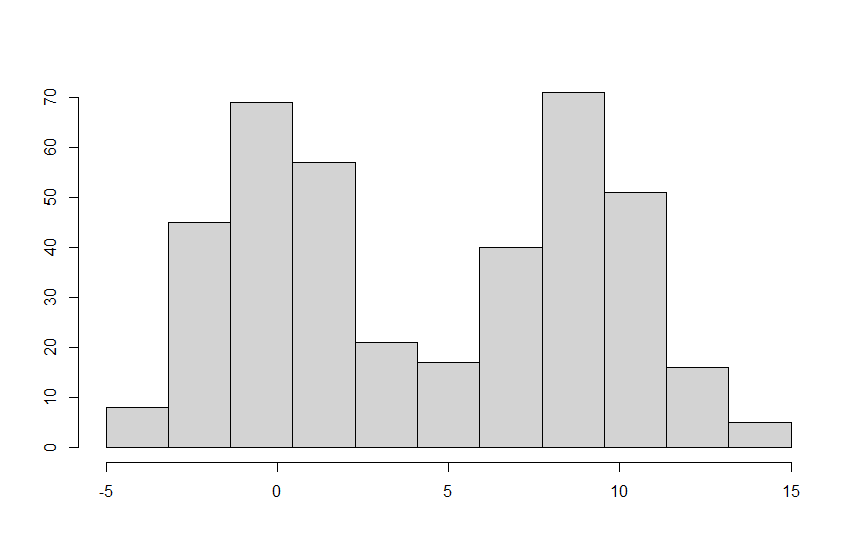
\includegraphics[width=10cm]{../fig/Cap02-DatosBimodales.png}
	\caption{Un conjunto de datos bimodal.}
	\label{cap02:fig:DatosBimodales}
    \end{figure}
El cálculo de la moda (o modas) es inmediato, a partir de las tablas de
frecuencias, y en los tutoriales comentaremos brevemente cómo realizarlo.

%\pendiente{Faltan ejemplos y un histograma bimodal para comparar con uno
%unimodal}

\section{Medidas de dispersión.}
\label{cap02:sec:MedidasDispersion}

%\subsection*{Introducción}

Hasta ahora hemos estado calculando {\em valores centrales}, que nos sirvieran
como buenos representantes de una colección de datos. Sin embargo, es fácil
entender que hay muchas colecciones de datos, muy distintas entre sí, que
pueden tener la misma media aritmética o la misma mediana, etcétera. El mismo
representante puede corresponder a colecciones de datos con {\em formas} muy
diferentes.

Por lo tanto, no sólo necesitamos un valor representativo, además necesitamos
una forma de medir {\em la calidad de ese representante.} ¿Cómo podemos hacer
esto? La idea que vamos a utilizar es la de \index{dispersión}{\sf dispersión}.
Una colección de números es poco dispersa cuando los datos están muy
concentrados alrededor de la media. Dicho de otra manera, si los datos son poco
dispersos, entonces se parecen bastante a la media (o al representante que
estemos usando). En una colección de datos poco dispersos, la {\em distancia
típica} de uno de los datos al valor central es pequeña.


Esa es la idea intuituiva, y como se ve está muy relacionada con el concepto de
{\em precisión} del que hablamos en la Sección
\ref{cap01:sec:PrecisionExactitudCifrasSignificativas} (ver la Figura
\ref{cap01:fig:PrecisionExactitud}, página
\pageref{cap01:fig:PrecisionExactitud}). Pero ahora tenemos que concretar mucho
más si queremos definir un valor de la dispersión que se pueda calcular. ¿cómo
podemos medir eso? En esta sección vamos a introducir varios métodos de medir
la dispersión de una colección de datos.

\subsection{Recorrido (o rango) y recorrido intercuartílico.}
\label{cap02:subsubsec:RangoIntercuartilico}

La idea más elemental de dispersión es la de \index{recorrido de una variable}{\sf recorrido}, que
ya hemos encontrado al pensar en las representaciones gráficas. El recorrido es simplemente la
diferencia entre el máximo y el mínimo de los valores. Es una manera rápida, pero excesivamente
simple, de analizar la dispersión de los datos, porque depende exclusivamente de dos valores (el
máximo y el mínimo), que pueden ser muy poco representativos. No obstante, es esencial, como primer
paso en el estudio de una colección de datos, empezar por calcular el recorrido, porque nos ayuda a
{\em enmarcar} nuestro trabajo, y evitar errores posteriores.

Un comentario sobre la terminología. El recorrido se denomina a veces, {\sf rango}\index{rango de
una variable}. Por razones que quedarán más claras en el Apéndice \ref{apendice:MasAlla}
(donde usaremos {\em rango} para otra noción distinta), nosotros preferimos el término {\em
recorrido} para este concepto. La confusión se debe a la traducción como {\em rango} de las dos
palabras inglesas {\em range}, que nosotros traducimos como {\em recorrido}, y {\em rank}, que
traducimos como {\em rango}.

Si queremos ir un paso más allá, para empezar a entender la forma de los datos, podemos usar las
medidas de posición. En concreto, la mediana y los cuartiles se pueden utilizar para medir la
dispersión de los datos, calculando el {\sf recorrido intercuartílico}\index{recorrido
intercuartílico} (en inglés, {\em interquartile range}, IQR) \index{IQR} \index{interquartile
range}, que se define como la diferencia entre el tercer y el primer cuartil.

        \begin{center}
            \fcolorbox{black}{Gris025}{\begin{minipage}{8cm}
            \begin{center}
            {\bf IQR, recorrido intercuartílico.}
            \end{center}
            El recorrido intercuartílico es:
            \[IQR=(\mbox{tercer cuartil}) - (\mbox{primer cuartil})\]
        \end{minipage}}
        \end{center}
\begin{ejemplo}
\label{cap02:ejem:IQR}
Para el conjunto de datos del Ejemplo \ref{cap02:ejem:MediaAritmetica02}, que eran estos:
\[9,\, 6,\, 19,\, 10,\, 17,\, 3,\, 28,\, 19,\, 3,\, 5,\, 19,\, 2,\, 150\]
el programa de ordenador (R, en este ejemplo) nos dice que el primer cuartil es $5$, y que el tercer cuartil es $19$. Por lo tanto,
\[IQR=19 - 5 = 14.\]
\qed
\end{ejemplo}

Los datos que son mucho menores que el primer cuartil o mucho mayores que el tercer cuartil se
consideran {\sf valores atípicos}\index{datos atípicos}\index{valores atípicos}\index{atípico} (en
inglés, {\em outlier})\index{outliers}. ¿Cómo de lejos tienen que estar de los cuartiles para
considerarlos {\em raros o excepcionales}? La forma habitual de proceder es considerar que {\sf un
valor mayor que el tercer cuartil, y cuya diferencia con ese cuartil es mayor que $1.5$ veces el
recorrido intercuartílico es un valor atípico}. De la misma forma, también es un valor atípico
aquel valor menor que el tercer cuartil, cuya diferencia con ese cuartil es mayor que
$1.5\cdot$IQR. Ya hemos discutido que existen muchas formas distintas de definir los cuartiles, así
que el recorrido intercuartílico depende, naturalmente, del método que se use para calcular los
cuartiles. Nosotros siempre lo calcularemos usando el ordenador (con R, la hoja de cálculo o algún
otro programa), y nos conformaremos con los valores por defecto que producen esos programas.

\begin{ejemplo}
\label{cap02:ejem:ValorAtipico}
Como habíamos anunciado, vamos a ver que, para el conjunto de datos del Ejemplo \ref{cap02:ejem:MediaAritmetica02}, el valor $150$ es un valor atípico. En el Ejemplo \ref{cap02:ejem:IQR} hemos visto que el tercer cuartil de esos valores era $19$, y que el recorrido intercuartílico era $14$. Así que un valor será atípico si es mayor que
\[\mbox{(tercer cuartil)}+1.5\cdot IQR=19 + 1.5 \cdot 14=19 + 21= 40.\]
Desde luego, queda claro que $150$ es un valor atípico, en ese conjunto.
\qed
\end{ejemplo}

La mediana, los cuartiles y el recorrido intercuartílico se utilizan para dibujar los diagramas
llamados de \index{diagrama de caja y bigotes} {\sf caja y bigotes} (en inglés,
{\em boxplot})\index{boxplot}, como el que se muestra en la Figura \ref{cap02:fig:Boxplot}. En estos
diagramas se dibuja una caja cuyos extremos son el primer y tercer cuartiles. Dentro de esa caja se
dibuja el valor de la mediana. Los valores atípicos se suelen mostrar como puntos individuales
(fuera de la caja, claro), y finalmente se dibujan segmentos que unen la caja con los datos más
alejados que no son atípicos.
    \begin{figure}[hp]
	\begin{center}
    (a)\\
	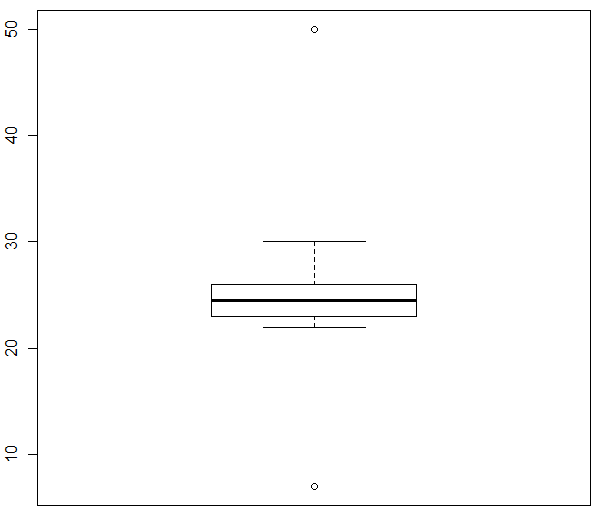
\includegraphics[width=9.5cm]{../fig/Cap02-BoxPlot.png}\\[3mm]
    (b)\\
    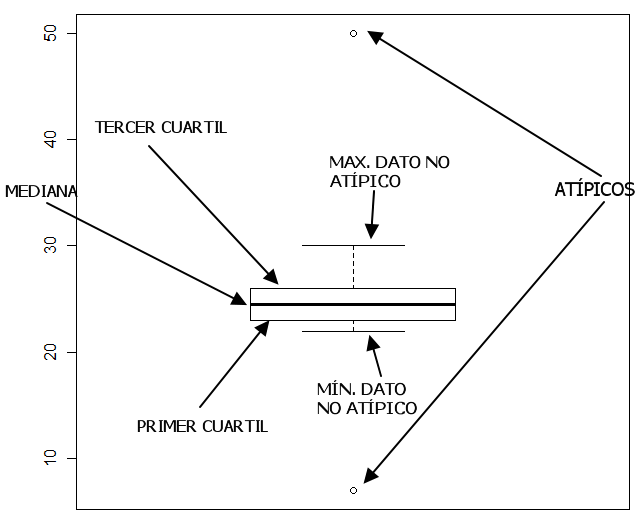
\includegraphics[width=10.5cm]{../fig/Cap02-BoxPlot-Estructura.png}
    \end{center}
	\caption{Un boxplot (a) y su estructura (b).}
	\label{cap02:fig:Boxplot}
    \end{figure}
Hasta hace muy poco, las hojas de cálculo no ofrecían la posibilidad de dibujar diagramas de cajas, y de hecho, nosotros recomendamos utilizar programas especializados para dibujarlos.
Aprenderemos a hacerlo en el Tutorial02, donde también veremos como calcular el recorrido
intercuartílico.

\subsection{Varianza y desviación típica.}
\label{cap02:subsec:VarianzaDesviacionTipica}

El recorrido intercuartílico se expresa en términos de cuartiles (o percentiles), y por lo tanto
tiene más que ver con la mediana que con la media aritmética. Sin embargo, uno de los objetivos más
importantes (si no el más importante) de la Estadística es hacer inferencias desde una muestra a la
población. Y cuando se trate de hacer inferencias, vamos a utilizar en primer lugar la media
aritmética como valor central o representativo de los datos. Por eso estas medidas de dispersión
relacionadas con la mediana, y no con la media, no son las mejores para hacer inferencia. {\sf
Necesitamos una medida de dispersión relacionada con la media aritmética.}

\subsubsection*{Varianza poblacional y cuasivarianza muestral.}


Tenemos, como siempre, un conjunto de $n$ datos,
\[x_1,x_2,\ldots,x_n\]
que corresponden a $n$ valores de una {\sf variable cuantitativa.} La primera
idea que se nos puede ocurrir es medir la diferencia entre cada uno de esos
valores y la media (la {\em desviación individual} de cada uno de los valores):
\[x_1-\bar x, x_2-\bar x,\ldots, x_n-\bar x,\]
Y para tener en cuenta la contribución de todos los valores podríamos pensar en hacer la media de estas desviaciones individuales:
\[\dfrac{(x_1-\bar x)+(x_2-\bar x)+\cdots+(x_n-\bar x)}{n}.\]
El problema es que esta suma siempre vale cero. Vamos a fijarnos en el numerador (y recuerda la definición de media aritmética):
\begin{equation}\label{cap02:ecu:SumaDesviacionesIgual0}
    (x_1-\bar x)+(x_2-\bar x)+\cdots+(x_n-\bar x)=(x_1+x_2+\cdots+x_n)-n\cdot\bar x=0.
\end{equation}
Está claro que tenemos que hacer algo más complicado, para evitar que el signo
de unas desviaciones se compense con el de otras. A partir de aquí se nos abren
dos posibilidades, usando dos operaciones matemáticas que eliminan el efecto de
los signos. Podemos usar el valor absoluto de las desviaciones individuales:
\[\dfrac{|x_1-\bar x|+|x_2-\bar x|+\cdots+|x_n-\bar x|}{n},\]
o podemos elevarlas al cuadrado:
\[\dfrac{(x_1-\bar x)^2+(x_2-\bar x)^2+\cdots+(x_n-\bar x)^2}{n}.\]
Las razones para elegir entre una u otra alternativa son técnicas: vamos a usar
la que mejor se comporte para hacer inferencias. Y, cuando se hacen inferencias
sobre la media, la mejor opción resulta ser la que utiliza los cuadrados. En
otros tipos de inferencia, no obstante, se usa la definición con el valor
absoluto.

La {\sf varianza (poblacional)} (o {\sf desviación cuadrática media})\index{varianza
(poblacional)}\index{desvici\'on cuadr\'atica media}\index{variance} (en ingl\'es, {\em variance})
del conjunto de datos $x_1,x_2,\ldots,x_n$ es:
        \begin{center}
        \fcolorbox{black}{Gris025}{
        \begin{minipage}{12cm}
                        \centering {\bf Varianza (poblacional).}
                        \begin{equation}\label{cap02:eq:varianzaPoblacional}
                    	  Var(x)=\dfrac{(x_1-\bar x)^2+(x_2-\bar x)^2+\cdots+(x_n-\bar x)^2}{n}=\dfrac{\displaystyle\sum_{i=1}^n(x_i-\bar x)^2}{n}.
                    	\end{equation}
        \end{minipage}}
        \end{center}
En muchos libros, incluso sin hablar de la varianza, se define una
cantidad relacionada, llamada {\sf varianza muestral} \index{varianza muestral}
o {\sf cuasivarianza muestral}, que es el nombre que nosotros vamos a usar,
\index{cuasivarianza muestral} mediante la fórmula
        \begin{center}
        \fcolorbox{black}{Gris025}{
        \begin{minipage}{12cm}
                        \centering {\bf Cuasivarianza muestral.}
                        \begin{equation}\label{cap02:eq:cuasivarianzaMuestral}
                    	  s^2(x)=\dfrac{(x_1-\bar x)^2+(x_2-\bar x)^2+\cdots+(x_n-\bar x)^2}{\colorbox{lightgrey}{$n-1$}}=\dfrac{\displaystyle\sum_{i=1}^n(x_i-\bar x)^2}{\colorbox{lightgrey}{$n-1$}}.
                    	\end{equation}
        \end{minipage}}
        \end{center}
Como puede verse, la única diferencia es que en el denominador de la fórmula
aparece $n-1$ en lugar de $n$. En particular, si $n$ es muy grande, ambas
cantidades son prácticamente iguales, aunque la cuasivarianza siempre es
ligeramente mayor.

El concepto de cuasivarianza muestral será importante cuando hablemos de
inferencia, y entonces entenderemos el papel que juega la cuasivarianza
muestral, y su relación con la varianza (poblacional) tal como la hemos
definido. Lo que sí es {\sf\large muy importante}, usando software o
calculadoras, es que sepamos si el número que se obtiene es la varianza o la
cuasivarianza muestral.

\begin{ejemplo}
\label{cap02:ejem:Varianza}
Para el conjunto de valores
\[9,\, 6,\, 19,\, 10,\, 17,\, 3,\, 28,\, 19,\, 3,\, 5,\, 19,\, 2,\]
del Ejemplo \ref{cap02:ejem:MediaAritmetica} (pág. \pageref{cap02:ejem:MediaAritmetica}), que ya hemos usado en varios ejemplos, su media aritmética es:
\[\bar x=\dfrac{140}{12}\approx 11.67.\]
Así que la varianza (poblacional) es:
\[Var(x)=\dfrac{\left(9-\frac{140}{12}\right)^2+\left(6-\frac{140}{12}\right)^2+\cdots+\left(19-\frac{140}{12}\right)^2+\left(2-\frac{140}{12}\right)^2}{12}=\]
\[=\dfrac{\frac{2360}{3}}{12}=\dfrac{2360}{36}\approx 65.56\]
con cuatro cifras significativas. La cuasivarianza muestral se obtiene dividiendo por $11$ en lugar de $12$, y es:
\[s^2=\dfrac{\left(9-\frac{140}{12}\right)^2+\left(6-\frac{140}{12}\right)^2+\cdots+\left(19-\frac{140}{12}\right)^2+\left(2-\frac{140}{12}\right)^2}{11}=\]
\[=\dfrac{\frac{2360}{3}}{11}=\dfrac{2360}{33}\approx 71.52,\]
también con cuatro cifras significativas.

Dejamos como ejercicio para el lector comprobar que, para los datos del Ejemplo \ref{cap02:ejem:MediaAritmetica02}, que incluyen el valor atípico $150$, la varianza poblacional y la cuasivarianza muestral son (con cuatro cifras significativas)
\[
Var(x)\approx 1419,\quad s^2\approx 1538.
\]
Como puede verse, con la presencia del valor atípico la dispersión del conjunto ha aumentado mucho.
\qed
\end{ejemplo}

\subsubsection*{Varianza a partir de una tabla de frecuencias.}

Cuando lo que tenemos son datos descritos mediante una tabla de frecuencias,
debemos proceder así:
\begin{enumerate}
    \item La Ecuación \ref{cap02:eq:varianzaPoblacional} se sustituye por:
%        \begin{center}
%            \fcolorbox{black}{Gris025}{ \centering {\bf Varianza
%            (poblacional) a partir de una tabla de frecuencias}
%
%            \begin{minipage}{12cm}
%                \[v=Var(x)=\dfrac{\displaystyle\sum_{i=1}^k\colorbox{lightgrey}{$\bf f_i\cdot$}(x_i-\bar x)^2}
%        	        {\colorbox{lightgrey}{$\bf \displaystyle\sum_{i=1}^k f_i$}}.\]
%            \end{minipage}
%            }
%        \end{center}
        \begin{center}
        \fcolorbox{black}{Gris025}{
        \begin{minipage}{12cm}
                        \centering {\bf Varianza (poblacional) a partir de
            una tabla de frecuencias.}
                        \[Var(x)=\dfrac{\displaystyle\sum_{i=1}^k\colorbox{lightgrey}{$\bf f_i\cdot$}(x_i-\bar x)^2}
        	        {\colorbox{lightgrey}{$\bf \displaystyle\sum_{i=1}^k f_i$}}.\]
        \end{minipage}}
        \end{center}





        donde, ahora, $x_1,\ldots,x_k$ son los valores {\em distintos} de la
        variable, y $f_1,\ldots,f_k$ son las correspondientes frecuencias.

    \item En el caso de datos agrupados por intervalos, los valores $x_i$
        que utilizaremos serán las marcas de clase.

\end{enumerate}
En los tutoriales tendremos ocasión sobrada de practicar este tipo de operaciones.


\subsubsection*{Desviación típica.}

La varianza, como medida de dispersión, tiene un grave inconveniente: puesto
que hemos elevado al cuadrado, las unidades en las que se expresa son
el cuadrado de las unidades originales en las que se medía la
variable $x$. Y nos gustaría que una medida de dispersión nos diera
una idea de, por ejemplo, cuantos metros se alejan de la media los
valores de una variable medida en metros. Dar la dispersión en metros
cuadrados es, cuando menos, extraño. Por esa razón, entre otras,
vamos a necesitar una nueva definición.

La {\sf desviación típica} \index{desviación típica} es la raíz
cuadrada de la varianza:
    \begin{center}
    \fcolorbox{black}{Gris025}{
    \begin{minipage}{12cm}
		\begin{center}
        {\centering \bf Desviación típica (poblacional).}
			\end{center}
            \[DT(x)=\sqrt{Var(x)} =\sqrt{\dfrac{\displaystyle\sum_{i=1}^n(x_i-\bar x)^2}{n}}.\]
        Y, si es a partir de una tabla de frecuencias, entonces:
                        \[DT(x)=\sqrt{\dfrac{\displaystyle\sum_{i=1}^k\colorbox{lightgrey}{$\bf f_i\cdot$}(x_i-\bar x)^2}
        	        {\colorbox{lightgrey}{$\bf \displaystyle\sum_{i=1}^k f_i$}}}.\]
    \end{minipage}}
    \end{center}
También existe una {\sf cuasidesviación típica muestral $s$}, que es la
raíz cuadrada de la cuasivarianza muestral, y con la que nos volveremos a encontrar muchas veces en el resto del curso.

El cálculo de la desviación típica tiene las mismas características que el de la varianza. Y, de
nuevo, es \underline{\sf muy importante}, usando software o calculadoras, que sepamos si el número
que se obtiene es la desviación típica o la cuasidesviación típica muestral.

\begin{ejemplo}
Para los datos del Ejemmplo \ref{cap02:ejem:Varianza}, y tomando raíces cuadradas, se obtiene una desviación típica poblacional aproximadamente igual a $8.097$ y una cuasidesviación típica muestral aproximadamente igual a $8.457$.
\qed
\end{ejemplo}
